%%%%%%%%%%%%%%%%%%%%
\newcommand{\functionANHTAO}[2]{
	\functionSignature{\texttt{anhtao-path}}{\varAtomicTask{}{}, \varAgent{}{}}
}

\subsection{The \acronymWSNOptimisationExtended{}{} algorithm}
\label{section:solution_anhtao}

\paragraph{Integrating \acronymWSNOptimisation{}{} into task paths}

The \acronymWSNOptimisation{}{} algorithm optimises utility of the system as described in Section \ref{section:energy_consumption}, Equation \ref{eq:system_utility}. 
To successfully complete a composite task, a sink must decompose the composite task it received from an external source into atomic tasks. It then selects whether to execute the tasks itself, or allocate them to further agents.  Figure \ref{fig:arc-flow}  illustrates how our algorithm fits into this process. It shows a task-path where there are two re-allocations made before a specific atomic task is allocated to an agent that completes the task by taking a measurement, then returns the results back along the task path.
\begin{figure}[ht]
	\centering
	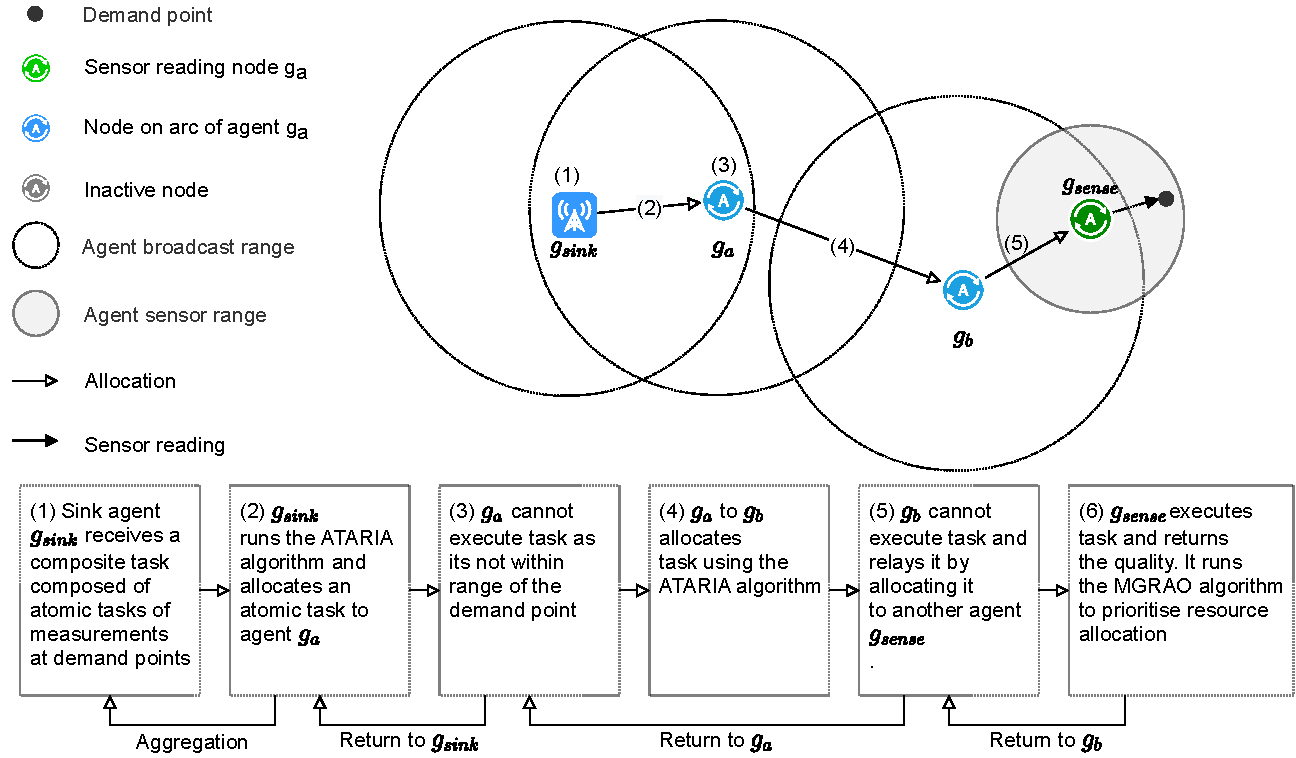
\includegraphics[width=0.8\linewidth, trim={72pt 0pt 62pt 0pt, clip}]{arc-flow}
	\caption{\textbf{Allocation along a task-path}. This diagram illustrates how allocations can be relayed along a task-path using successive applications of the \acronymATARIA{}{} algorithm.}
	\label{fig:arc-flow}
\end{figure}

\paragraph{Optimisation using \acronymWSNOptimisation{}{}}

The \acronymWSNOptimisation{}{} algorithm optimises this process  in 3 main ways;
\begin{enumerate}
	\item \textit{Selecting actions.} When agents have a composite or atomic task allocated to them, they can choose from a range of actions. By utilising Q-learning techniques, with absolute task values as the reward function, \acronymWSNOptimisation{}{} adapts the probability of agents' taking actions to optimise these values. 
	
	\item \textit{Resource allocation.} As an agent completes an atomic task it will use some resources to do so. The \acronymWSNOptimisation{}{} algorithm predicts the agents' optimal allocation of these resources, given the different atomic tasks it is allocated, and their distribution over time. This allows it to complete the incoming tasks to obtain best atomic task values overall.
	
	\item \textit{Forming task-paths. }The algorithm allows agents to re-allocate atomic tasks to other agents, relaying them through the network.  It also distributes the reward for completing these tasks across agents in these task paths to optimise the actions that were taken by all agents that participated in the task.
\end{enumerate}
The high-level flowchart in Figure \ref{fig:algorithm-flow}(a) shows how sinks decompose composite tasks, choose actions to take, allocate atomic tasks, and return results. In Figure \ref{fig:algorithm-flow}(b) we can see how agents in a task-path choose actions, and how they execute or re-allocate the atomic tasks they have been allocated.
\begin{figure}[ht]
	\centering
	\begin{subfigure}{0.75\textwidth}
		\centering
		\caption{Sink agent flow}
		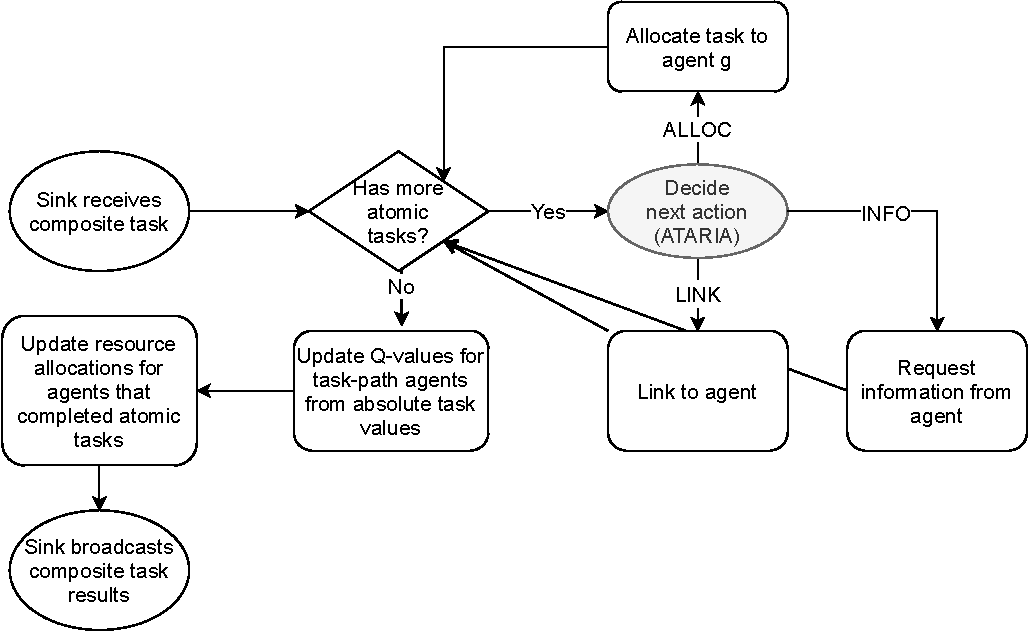
\includegraphics[width=0.9\linewidth, trim={25pt 0pt 25pt 0pt, clip}]{algorithm-flow-sink}
		\label{fig:algorithm-flow-sink}
	\end{subfigure} \hfill%
	\begin{subfigure}{0.75\textwidth}
		\caption{Task-path agent flow}
		\centering	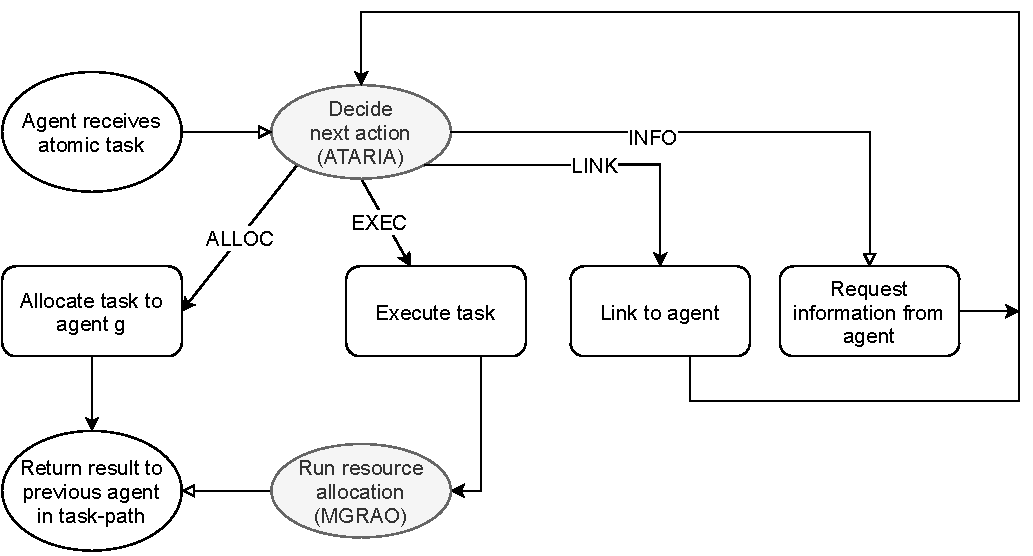
\includegraphics[width=0.9\linewidth,trim={25pt 0pt 25pt 0pt, clip}]{algorithm-flow-arc}
		\label{fig:algorithm-flow-arc}
	\end{subfigure}
	\caption{\textbf{\acronymWSNOptimisation{}{} execution flowchart.} Shows how \acronymWSNOptimisation{}{} combines the \acronymATARIA{}{} and \acronymMGRAO{}{} algorithms and enables recursive allocation of tasks.}
	\label{fig:algorithm-flow}
\end{figure}

\paragraph{High-level description of  \acronymWSNOptimisation{}{}}

We separate  the \acronymWSNOptimisation{}{} algorithm in two parts for clarity, the \acronymWSNOptimisationSink{}{} and \acronymWSNOptimisationArc{}{} algorithms. These are shown in Algorithms \ref{alg:wsn_optimisation_sink} and \ref{alg:wsn_optimisation_arc} respectively. 

\begin{itemize}
	\item[]  \textbf{\acronymWSNOptimisationSink{}{}} Initially, the sink receives a composite task $\varCompositeTask{}{}$ comprising of multiple atomic tasks $\varAtomicTask{}{}$ to be completed. While these atomic tasks are not yet completed or allocated, the  \acronymATARIA{}{} algorithm runs to select an action for the sink (Line \ref{wsnsink:select}).  If the action chosen is for the sink to execute the atomic task itself, $\functionExec{}{}$, the algorithm uses the \acronymMGRAO{}{} algorithm to determine the resources that are allocated to that task types' completion. An $\functionAlloc{}{}$ action will allocate the task to another agent it knows about to complete using the \acronymWSNOptimisationArc{}{} algorithm. In both cases, the task is removed from the list of active tasks  (Line \ref{wsnsink:exec_remove}). If a $\functionInfo{}{}$ or $\functionLink{}{}$ action is executed, these will update the agents' neighbourhood and knowledge base respectively using the \acronymATARIA{}{} algorithm. There is no effect on atomic task execution or allocation in that case, and the algorithm loops round to choose another action. The selection and execution of actions using the \acronymATARIA{}{} algorithm is repeated until the tasks are either executed or allocated. Once all the atomic tasks are allocated, the sink must wait for them to complete (Line \ref{wsnsink:wait}). 
	
	When all the atomic tasks in the composite task have completed, each atomic tasks' absolute task value is calculated (Line \ref{wsnsink:ataria-taskval}). All of the agents in each atomic tasks' task-path have their Q-values updated using these values, acting as reward values for the actions they took in completing each task (Line \ref{wsnsink:ataria-update}). Finally, for each atomic task, the corresponding absolute task value is used by each agent that completed the task, to update its allocation of resources using the \acronymMGRAO{}{} algorithm (Line \ref{wsnsink:mgrao}).

	\item[] \textbf{\acronymWSNOptimisationArc{}{}} This part of the algorithm will complete an atomic task and return its quality, either by executing the task itself, or re-allocating to another agent.  Once again,  the \acronymATARIA{}{} algorithm is used to repeatedly select actions until the atomic task is either completed by  self-execution or allocated (Line \ref{wsnarc:select}). After waiting for the atomic task to be completed (Line \ref{wsnarc:wait}),  an atomic task quality is returned (Line \ref{wsnarc:wait}).
\end{itemize}
 \begin{algorithm}[ht]
	\DontPrintSemicolon
	\footnotesize
	
	\caption{\textbf{The \acronymWSNOptimisationSink{}{} algorithm}}
	\label{alg:wsn_optimisation_sink}
	{
		\KwIn{ $\varCompositeTask{}{}$ , The composite task set}
		\KwIn{ $\varAgent{}{}$ , The sink completing the composite task}
		\KwResult{$\functionCompositeTaskQuality{}{}{}{}$ , The composite task quality of $\varCompositeTask{}{}$}		\nonl \;
		\tcp{Copy set of atomic tasks to list of incomplete tasks}
		$ctactive \leftarrow \varCompositeTask{}{}$ \label{wsnsink:copy}\;
		\ForEach{$\varAtomicTask{}{} \in ctactive$\label{wsnsink:composite_tasks}}
		{
			\tcp{Select and execute action through \acronymATARIA{}{}}
			$\varAction{}{} \leftarrow \functionATARIAAction{}{}$ \label{wsnsink:select} \;	
			\If{$\functionAgentActionType{}{} = \functionExec{}{} \lor  \functionAgentActionType{}{} = \functionAlloc{\varAtomicTask{}{}}{\varAgent{}{'}}$?}
			{
				\tcp{If the action was completed by agent $\varAgent{}{}$ or by allocating to another agent $\varAgent{}{'}$, remove atomic task from active task list}
				$ctactive{}{} \leftarrow ctactive - \lbrace \varAtomicTask{}{} \rbrace$ \label{wsnsink:exec_remove}\;
			}
		}
		\tcp{Wait for all the atomic tasks in the composite task to be completed}
		\While{ $\functionNotComplete{\varCompositeTask{}{}}{}$}{
			$\functionWait{}{}$ \label{wsnsink:wait}\; 
		}
		\ForEach{$\varAtomicTask{}{} \in \varCompositeTask{}{}$\label{ataria:composite_tasks}}
		{
			\tcp{Calculate each atomic tasks' absolute task value}
			$\varTaskValue{}{} \leftarrow \functionTaskAbsoluteValue{}{}
			$ \label{wsnsink:ataria-taskval}\;	
			\tcp{Send a proportion of the absolute task value for the atomic task to each agent in its task-path}
			\ForEach{$\varAgent{}{'}\in \functionTaskArc{}{}$}{
				\tcp{Update the Q-values for actions taken by agents in each atomic tasks' task-path}
				$\functionSignature{\texttt{ataria-update}}{
					\varAgent{}{'}, \varAtomicTask{}{}, \frac{\varTaskValue{}{}}{\funcSize{\varCompositeTask{}{}}}
				}$ \label{wsnsink:ataria-update}\;	
			}
			\tcp{Send the agent that completed the atomic task the absolute task value to run the MGRAO update}
			$\functionSignature{\texttt{mgrao-update}}{\functionSinkRole{}{}, \varAtomicTask{}{}, \varTaskValue{}{}}$ \label{wsnsink:mgrao}\;	
		}
		\Return{$\functionCompositeTaskQuality{}{}{}{}$}
	}
\end{algorithm}
\begin{algorithm}[ht]
	\DontPrintSemicolon
	\footnotesize
	
	\caption{\textbf{The \acronymWSNOptimisationArc{}{} algorithm } }
	\label{alg:wsn_optimisation_arc}
	{
		\KwIn{ $\varAtomicTask{}{}$ , The atomic task to be completed}
		\KwIn{ $\varAgent{}{}$ , The agent completing the atomic task}
		\KwResult{$\functionAtomicTaskQualitySignature{}{}$ , The atomic task quality of $\varAtomicTask{}{}$}
		\nonl \;
		
		$taskAllocated \leftarrow False$ \;
		\While{$\neg taskAllocated$ }{
			\tcp{Select and execute action through \acronymATARIA{}{}}
			$\varAction{}{} \leftarrow \functionATARIAAction{}{}$ \label{wsnarc:select} \;
			\tcp{If the action was executed by agent $\varAgent{}{}$ or allocated to another agent $\varAgent{}{'}$, mark it allocated}
			\uIf{$\functionAgentActionType{}{} = \functionExec{}{} \lor \functionAgentActionType{}{} = \functionAlloc{\varAtomicTask{}{}}{\varAgent{}{'}}$?}
			{
				$taskAllocated \leftarrow True$ \;
			}
		}
		\tcp{Wait for the atomic task to be completed}
		\While{ $\functionNotComplete{\varAtomicTask{}{}}{}$}{
			$\functionWait{}{}$ \label{wsnarc:wait}\; 
		}
		\tcp{Return the task quality of the atomic task completion}
		\Return{$\functionAtomicTaskQualitySignature{}{}$\label{wsnarc:return}} \;
	}
\end{algorithm}